\documentclass[a4paper]{article}
\usepackage[utf8]{inputenc}
\usepackage{graphicx}
\usepackage{fullpage}
\usepackage{amsmath}
\usepackage{caption}
\usepackage{subcaption}
\usepackage[hidelinks, colorlinks=true, urlcolor=blue, linkcolor=black]{hyperref}

\title{Implementing Residual Connection on QCNN architecture}
\author{
Mini Project - \emph{CS-2-14(PO)}  \\\\  \small{By} \\\\  Krishiv Trivedi\hspace{0.2cm} [2023UMA0218] \\ Piyush Kumar \hspace{0.193cm} [2023UMA0227] \\ Krishna \hspace{1.58cm}[$2023UEE0140$] \\ Jyoti Yadav \hspace{0.86cm}[$2023UEE0139$] \\\\ \small{Supervisor:} \\ Sumit Kumar Pandey \\ \hspace{0.94cm}\\
}
\date{$12^{th}$April, 2025}
\begin{document}
\maketitle
\hrule
\section*{Introduction}
Quantum computing is a new computing paradigm based on quantum
mechanics that utilizes qubits instead of classical bits to store and process
information. Quantum nature like superposition and entanglement aren't just theoretical figments, now with the capacity to actually engineer these quantum systems, this nature can be meaningfully utilized and harnessed to speed up NP Algorithms like ``\emph{Brute-Force} \emph{\textbf{Knapsack}}''\footnote{[https://en.wikipedia.org/wiki/Knapsack\_problem]} and the ``\emph{\textbf{Travelling Salesman Problem}}'' (TSP) and improve our modern AI models.\\

 While the majority of our journey includes learning about theory of quantum circuits, learning and developing our own quantum algorithms for solving TSP etc. Our final aim of this paper will be the upcoming, \emph{Quantum Convolutional Neural Networks} (\textbf{QCNNs})\footnote{[https://pennylane.ai/qml/glossary/qcnn]}. We will demonstrate not only of how we can use the `Quantum' to develop better convolutional neural networks but also show an implimentation of a quantum circuit-based algorithm, \emph{quantum residual neural networks}\footnote{[https://doi.org/10.1038/s42005-024-01719-1]}.\\

Finally, we will explain what we have learnt so far from this vast theory and then display the different results produced by a Classical CNN and a Quantum CNN. The results will on a fixed dataset for both the networks, and display the differences in the important parameters like accuracy, cost function trends and our current engineering limitations on implemetation of QCNNs.

\section*{Motivation}
In this new quantum era, as the number of qubits increase and our engineering catches up to our theory, the security of our existing cryptographic methods is starting to diminish. The main motivation for this project was `\textbf{Post-Quantum Cryptography}'. Later, we transposed from ``How to make a problem which cannot be efficiently cracked by a quantum computer...'' to ``All such problems which can be efficiently cracked by a quantum computer...'' where we encountered many NP hard problems but first we focused on a known solved problem of `Knapsack' after which we started to develop our own algorithm with all that we have learnt for TSP.
\begin{itemize}
\item[Q.] How does a Quantum Computer solve such ``\emph{Brute-force}'' problems `\emph{faster}'?
\item[\textbf{$\rightarrow$}] We will not elaborate on the theory as to keep this report concise. While we have to classically iterate over all solutions to check, in quantum we use the \textbf{\emph{Hadamard}}\footnote{[https://en.wikipedia.org/wiki/Quantum\_logic\_gate]} Gate to check all such superpositions simultaneously.\vspace{5pt}\\
This is used extensively in quantum algorithms. Our main focus was on how to make the brute-force solution $O(2^{n})$ more optimal, which we did using \emph{\textbf{Grovers' Algorithm}}\footnote{[https://en.wikipedia.org/wiki/Grover\%27s\_algorithm]} which reduced the complexity to $O(2^{n/2})$. In general, we can say that in such brute-force approaches, Grovers provides a well-known $\sqrt{N}$ ``quadratic-speedup''.

\item[Q.] Why did we choose \emph{QCNNs}/\emph{QRNNs}?
\item[\textbf{$\rightarrow$}] We think that making a hands-on quantum circuit in a domain which has practical implications in the future of machine learnning and AI will not only show how we can turn our theoretical knowledge into practice, which is the best way to display what we have learnt, but also simultaneously work on the edge of scientific innovation happening in the field of quantum computing as we speak. This is why we will be implementing a very recent paper published in 2024 as our contribution to this field of research.

\item[Q.] What do we actually use, software or anything to implement and run these quantum algorithms and get results?
\item[\textbf{$\rightarrow$}] While we do not have a quantum computer,  \emph{IBM's} quantum cloud computing provides us few qubits to work with. For this we are further using \textbf{\emph{Qiskit}} to simulate qubits, even if due to the nature of qubits it gets difficult to simulate more than 14-15 qubits at a time on a classical computer, we can simulate for our use case.
\end{itemize}

\section*{Methodology \& Implementation Idea}

For our methodology, first we'll make a Quantum CNN on a particular dataset, after which we will make an equivalent Classical CNN and compare the results to see which one performs better and their cost function trends. After this, we will implement the `Residual-block' into our QCNN to see the difference it produces. 
\begin{itemize}
\item \textbf{Dataset} consists of all tic-tac-toe games which have not ended in a draw. This dataset is actually very complex compared to all the dataset which a QCNN is typically trained on, i.e. detecting horizontal/vertical stripes on a 2x2 or a 4x2 grid, but we decided to push the limits of current standards. This is because we wanted to make a QCNN model never made before.

\begin{figure}[h]
\centering
\begin{subfigure}{.5\textwidth}
  \centering
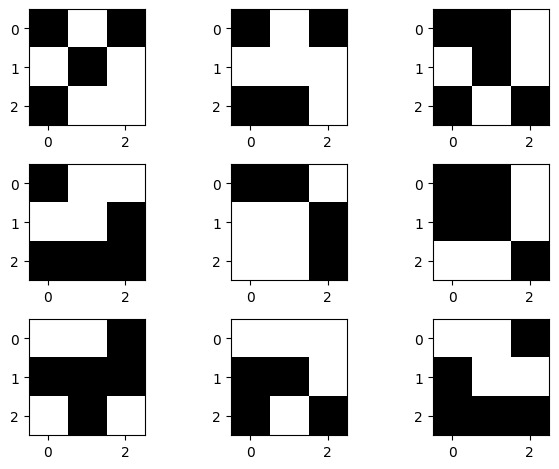
\includegraphics[height = 0.5\textwidth]{assets/dataset.jpeg}
  \label{fig:sub1}
\end{subfigure}%
\begin{subfigure}{.5\textwidth}
  \centering
  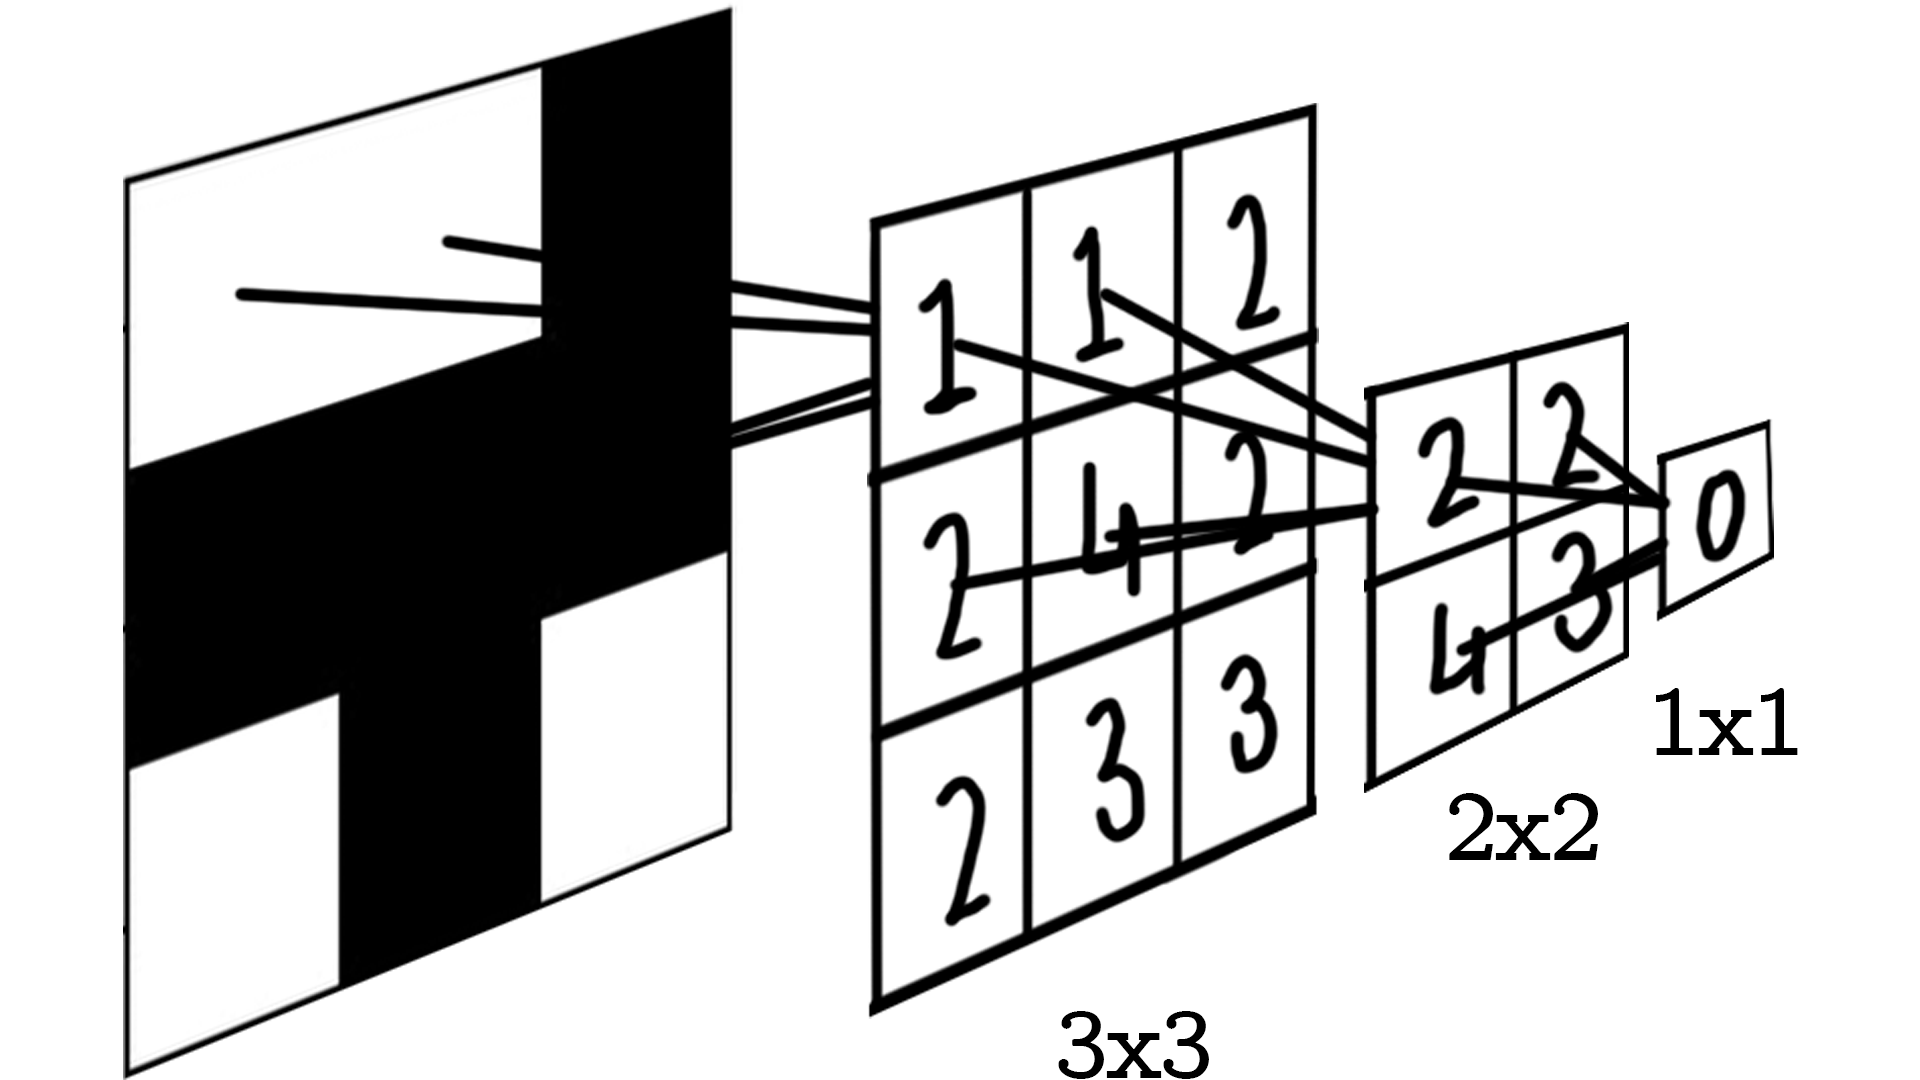
\includegraphics[height=.5\linewidth]{assets/CCNN.png}
  \label{fig:sub2}
\end{subfigure}
\caption{Our generated dataset and the overarching convolution model for both variations.}
\label{fig:test}
\end{figure}

\item \textbf{Layers} of pure convolutional networks are used. First is a convolution of a $3\times3$ to another $3\times3$ matrix, we'll call it $C_{3\times3}$. Next is a pooling layer from $3\times3$ to $2\times2$, we'll call it $P_{3\times3,2\times2}$. Similarly $C_{2\times2}$, $P_{2\times2,1\times1}$. The only difference is that the QCNN model uses an additional $P_{2\times2,2\times1}$ and $C_{2\times1}$ before pooling back via $P_{2\times1,1\times1}$.
\[\text{\emph{\textbf{CCNN}}: Input} \rightarrow C_{3\times3} \rightarrow P_{3\times3,2\times2} \rightarrow C_{2\times2} \rightarrow P_{2\times2,1\times1} \rightarrow \text{Output}\]
\[\text{\emph{\textbf{QCNN}}: Input} \rightarrow C_{3\times3} \rightarrow P_{3\times3,2\times2} \rightarrow C_{2\times2} \rightarrow P_{2\times2,2\times1} \rightarrow C_{2\times1} \rightarrow P_{2\times1,1\times1} \rightarrow \text{Output}\]

\begin{figure}[h]
\centering
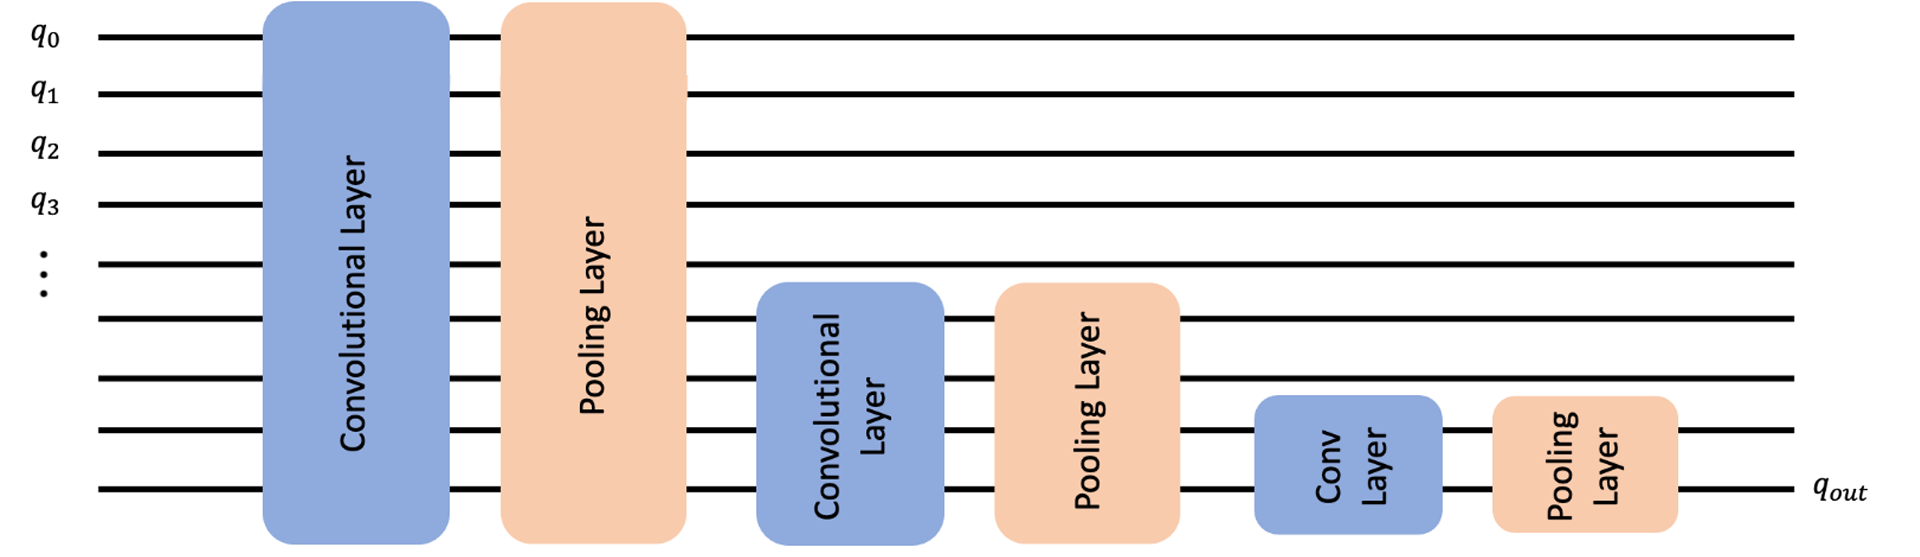
\includegraphics[height = 0.3\textwidth]{assets/QCNN.png}
\label{fig:test}
\end{figure}

\item \textbf{Training} of CCNN was done with Adam optimizer [\emph{PyTorch}], Cost-function: Cross Entropy. QCNN was with COBYLA optimizer [\emph{Qiskit}]\footnote{[https://docs.quantum.ibm.com/api/qiskit/0.27/qiskit.algorithms.optimizers.COBYLA]}, Cost-function: Squared Error (Default).

\begin{figure}[h]
\centering
\begin{subfigure}{.2\textwidth}
  \centering
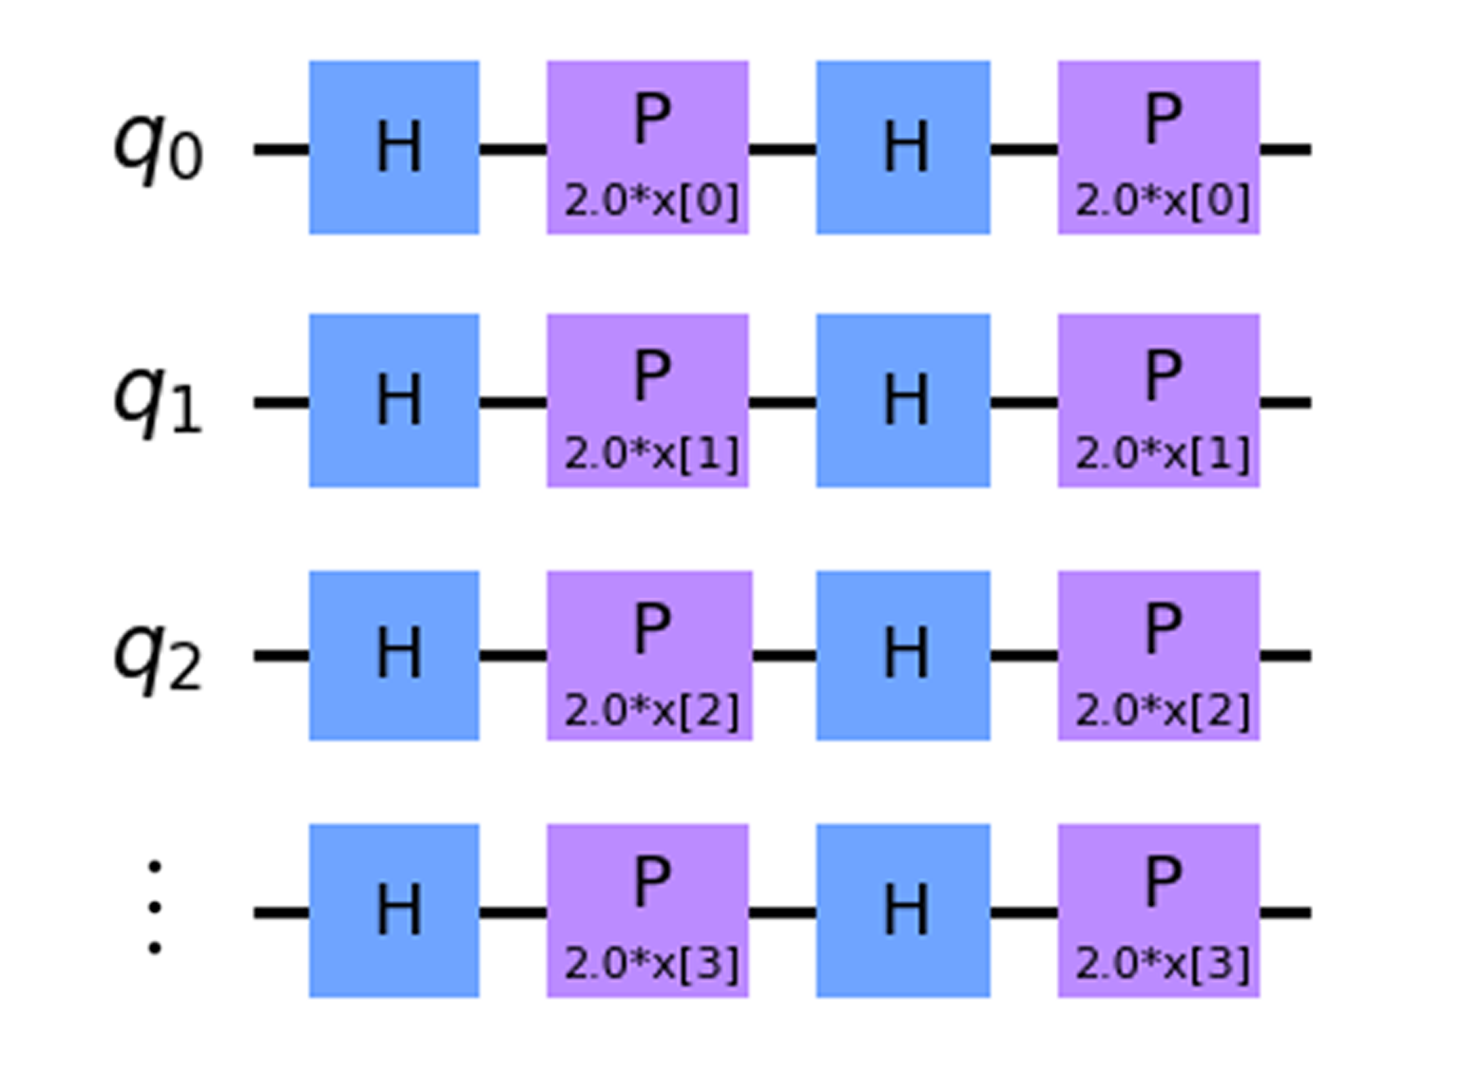
\includegraphics[height = 0.7\textwidth]{assets/zfm.png}
  \caption{ZFeatureMap}
  \label{fig:sub1}
\end{subfigure}%
\begin{subfigure}{.2\textwidth}
  \centering
  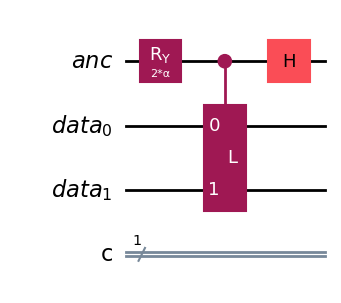
\includegraphics[height=.7\linewidth]{assets/rb.png}
  \caption{$\mathcal{R}(x)$}
  \label{fig:sub2}
\end{subfigure}%
\begin{subfigure}{.2\textwidth}
  \centering
  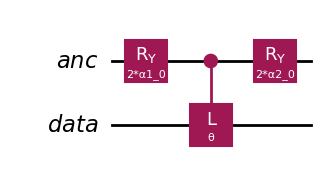
\includegraphics[height=.7\linewidth, width=.9\linewidth]{assets/r2.png}
  \caption{$\mathcal{R}_2(x)$}
  \label{fig:sub2}
\end{subfigure}%
\begin{subfigure}{.2\textwidth}
  \centering
  \includegraphics[height=.7\linewidth, width=1.\linewidth]{assets/conv\_element.png}
  \caption{$C$ Layer element}
  \label{fig:sub2}
\end{subfigure}%
\begin{subfigure}{.2\textwidth}
  \centering
  \includegraphics[height=.7\linewidth]{assets/pool\_element.png}
  \caption{$P$ Layer element}
  \label{fig:sub2}
\end{subfigure}%
\label{fig:test}
\end{figure}
\item \textbf{Additional} blocks were added like ZFeatureMap\footnote{[https://docs.quantum.ibm.com/api/qiskit/qiskit.circuit.library.ZFeatureMap]} before sending them to the layers to encode the data into qubits. And then we built and added our `Residual-Blocks' from the 2024 paper.
\end{itemize}
This is the method we have chosen to implement this quantum circuit. Our main focus in this paper is to show a detaied and practical implementation so we'll skip the intuition and theory which comes with this. Next is to report the results by both of these models [\emph{Now uploaded on \href{https://github.com/f361015/Quantum-CNN-TicTacToe}{GitHub}}].\footnote{Please see the references for the theoritical aspect, you won't be dissapointed!}

\section*{Results}

For our Classical CNN, we understand that with our cross entropy function and Adams Optimizer which are all well developed systems when it comes to CNN gives our Classical model a huge advantage.

\begin{itemize}
\item[$\Rightarrow$] \textbf{Accuracy}: 81.5 $\pm$ 1\%
\item[$\Rightarrow$] \textbf{Epochs}: 300
\end{itemize}

Similarly for the same dataset and same architecture for our QCNN model. Note that this comparision is purely with our convolutional QCNN and is without the use of $\mathcal{R}(x)$ and $\mathcal{R}_2(x)$ blocks.

\begin{itemize}
\item[$\Rightarrow$] \textbf{Accuracy}: 77\%
\item[$\Rightarrow$] \textbf{Epochs}: 200
\end{itemize}
\newpage

\begin{figure}[h]
\centering
\begin{subfigure}{.5\textwidth}
  \centering
  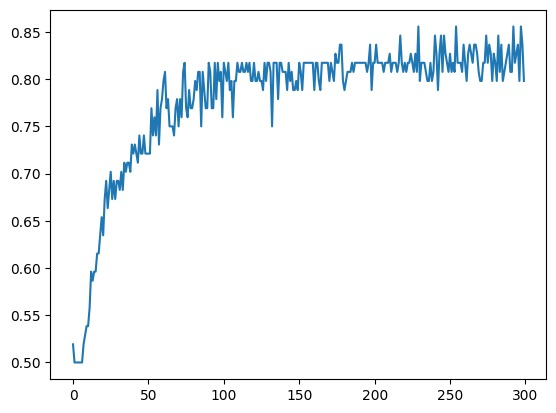
\includegraphics[height=0.7\linewidth]{assets/accu.jpeg}
  \caption{CCNN Accuracy}
  \label{fig:sub1}
\end{subfigure}%
\begin{subfigure}{.5\textwidth}
  \centering
  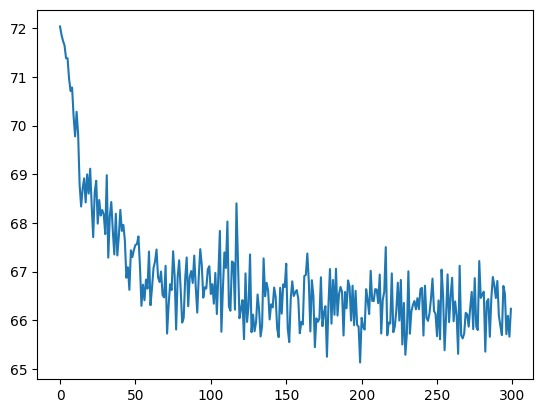
\includegraphics[height=.7\linewidth]{assets/cf.jpeg}
  \caption{CCNN Cross Entropy Loss}
  \label{fig:sub2}
\end{subfigure}%
\caption{Results of Classical CNN}
\label{fig:test}
\end{figure}
Now, we use the `Residual-Blocks' to see the difference between QCNN with and without the residual connection architecture.

We also made another improvement in our residual QCNN, that is, diagonally entangling the qubits to also capture the diagonal features of this dataset. You can see the full circuit in the GitHub repo, rest all the components of the QCNN are compeletely the same. Now the results of just adding one layer of Residual Blocks is as follows.

\begin{itemize}
\item[$\Rightarrow$] \textbf{Accuracy}: 81.73\%
\item[$\Rightarrow$] \textbf{Epochs}: 300
\end{itemize}

\begin{figure}[h]
\centering
\begin{subfigure}{.5\textwidth}
  \centering
  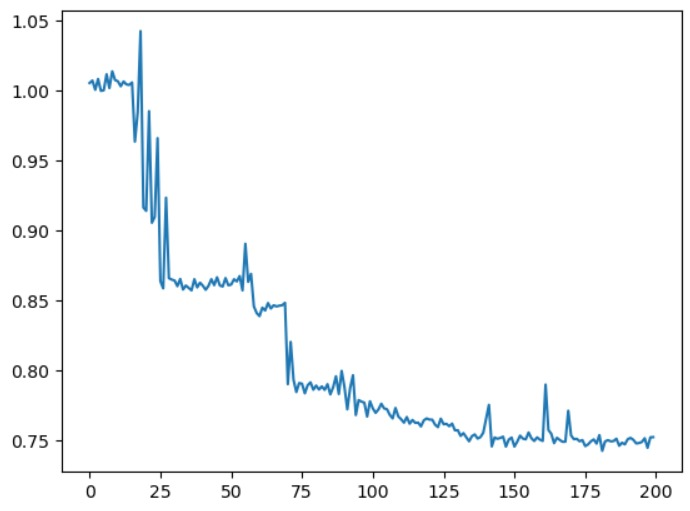
\includegraphics[height=0.7\linewidth]{assets/qcnn.jpeg}
  \caption{QCNN Sqrd.Error Loss wo/Residual Blocks}
  \label{fig:sub3}
\end{subfigure}%
\begin{subfigure}{.5\textwidth}
  \centering
  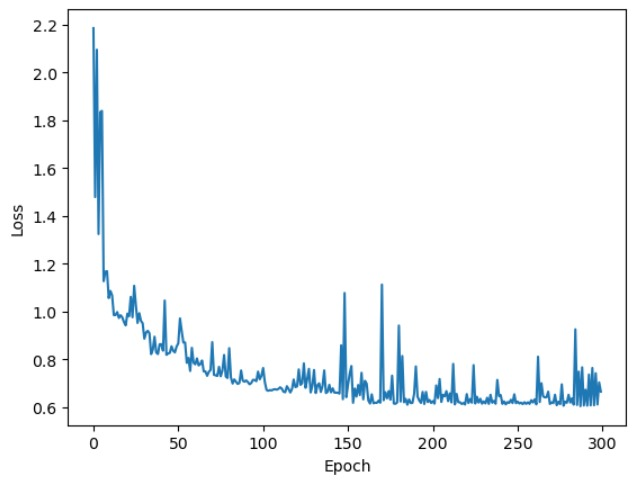
\includegraphics[height=.7\linewidth]{assets/imp_qcnn.jpeg}
  \caption{QCNN w/Residual Blocks}
  \label{fig:sub2}
\end{subfigure}%
\caption{Results of Quantum CNN}
\label{fig:test}
\end{figure}%
\section*{Conclusion \& Future}

Our Non-residual QCNN model reaches almost the same accuracy the CCNN reaches in 100 epochs. With more computing and time we might be able to replace CCNN with negligible decrease in performance. Also, the point to be noted is that our code is just simulating the qubits which makes it slower than if we had a actual quantum computer.\\

Meanwhile, our Improved-Residual-QCNN challenges our current Classical CNN! This small improvement and adding residual-blocks has made a significant breakthrough!

\begin{itemize}
\item[Q.] \textbf{\emph{So, What improved}}?
\item[\textbf{$\rightarrow$}] We hypothesized that it is mostly to do with the ``\emph{Diagonal wins of a player}'', this is because, when we analyzed all the games that our quantum model got wrong, we see that it was only the games where the wins were diagonal.

That is, the model correctly predicted all horizontal and vertical wins correctly. In case of diagonal cases...
\[ \text{\textbf{Correct}: } 32/56 \text{ \textbf{Incorrect}: } 24/56 \]
So we think the diagonalization due to the ``Residual-Blocks'' and convolution layers made it so that our new QCNN was good at identifying those extra features. Our new and improved model however, has only 19 incorrect diagonals.
\end{itemize}
\begin{figure}[h]
\centering
\begin{subfigure}{.5\textwidth}
  \centering
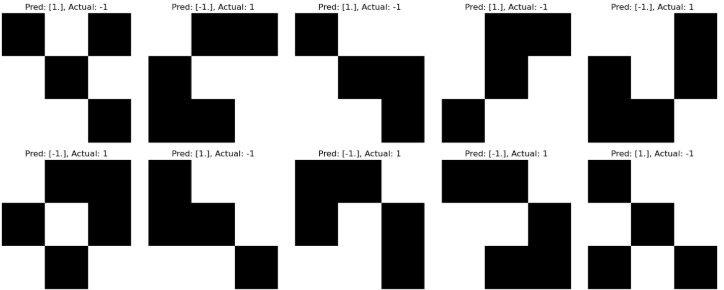
\includegraphics[height = 0.4\textwidth]{assets/2.jpeg}
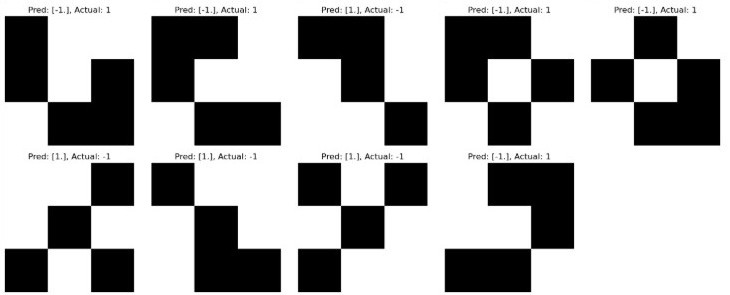
\includegraphics[height = 0.4\textwidth]{assets/1.jpeg}
\end{subfigure}%
\begin{subfigure}{.5\textwidth}
  \centering
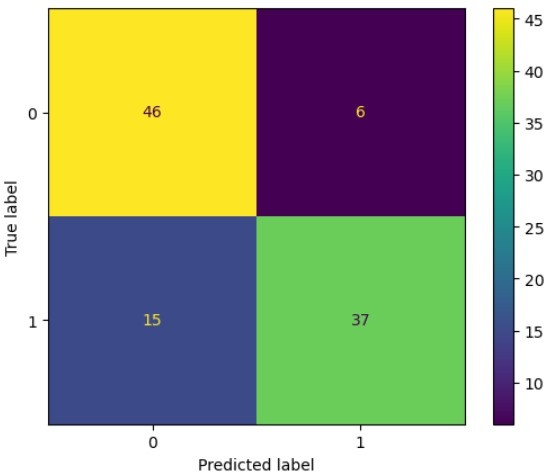
\includegraphics[height = 0.8\textwidth]{assets/confmat.jpeg}
\end{subfigure}%
\end{figure}%

Our future prospects include making a multi-classification model. For example, a model which detects if a game is won by white or black or is a draw. We already partially have the multimodel ready on hand if you need for demonstration.\\

\indent \textbf{Literature Review \& References: }
\begin{itemize}
\item Wen, J., Huang, Z., Cai, D. et al. Enhancing the expressivity of quantum neural networks with residual connections. Commun Phys 7, 220 (2024).
\item https://pennylane.ai/qml/glossary/qcnn
\item https://docs.quantum.ibm.com/api/qiskit/0.27/qiskit.algorithms.optimizers.COBYLA
\item https://docs.quantum.ibm.com/api/qiskit/qiskit.circuit.library.ZFeatureMap
\item https://en.wikipedia.org/wiki/Grover\%27s\_algorithm
\item https://en.wikipedia.org/wiki/Knapsack problem
\item https://en.wikipedia.org/wiki/Quantum\_logic\_gate

\end{itemize}

\end{document}